\documentclass[tikz,border=6pt]{standalone}
\usetikzlibrary{arrows.meta,positioning}
\begin{document}
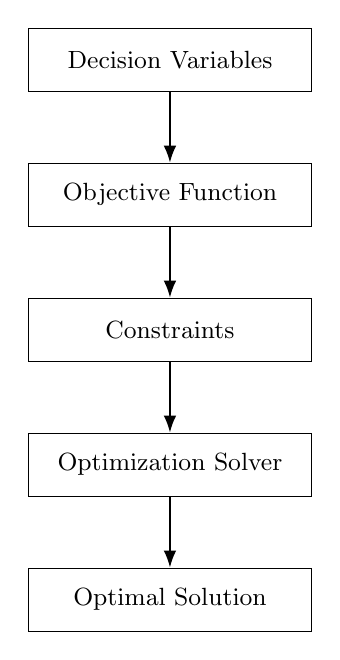
\begin{tikzpicture}[
  block/.style={draw, rectangle, minimum width=36mm, minimum height=8mm, align=center, font=\small},
  arrow/.style={-Latex, line width=0.7pt},
  node distance=9mm
]
\node[block] (vars) {Decision Variables};
\node[block, below=of vars] (obj) {Objective Function};
\node[block, below=of obj] (con) {Constraints};
\node[block, below=of con] (solver) {Optimization Solver};
\node[block, below=of solver] (result) {Optimal Solution};
\draw[arrow] (vars) -- (obj);
\draw[arrow] (obj) -- (con);
\draw[arrow] (con) -- (solver);
\draw[arrow] (solver) -- (result);
\end{tikzpicture}
\end{document}
